\chapter{多项式的根}
多项式的根是一个重要的概念,也是我们研究的主要问题之一,本章在复习的基础上,将系统地研究多项式的整数根,有理数根,实数根的存在、判定和计算方法。

\section{多项式的根及求根公式}
我们已经知道,如果当$x=a$时,多项式的值$f(a)=0$, 就把数值$a$叫做多项式$f(x)$的一个根,或叫做多项式函数$f(x)$的一个零点。

显然,零次多项式$f(x)=b\ne 0$, 没有任何根;零多项式$f(x)=0$有无限多个根(任意数都是它的根)。

因此,一元$n$次多项式
\[f(x)=a_nx^n+a_{n-1}x^{n-1}+\cdots+a_1x+a_0\quad (a_n\ne 0)\]
的根,就是一元$n$次方程
\[a_nx^n+a_{n-1}x^{n-1}+\cdots+a_1x+a_0=0\]
的根。求多项式的根,就是解相应的方程式。

要求多项式的根,首先应明确在那一个数系范围内,因为多项式和方程一样,同一个多项式在不同的数系范围内,可能会有不同的根存在。

在此,我们主要讨论和计算多项式的实数根,对其中更容易研究的有理系数多项式的有理根及整系数多项式的整数根更要特别讨论。

\subsection{一元一、二次多项式的求根公式}

一元一次、一元
二次多项式的求根公式也就是一元一次、一元二次方程的求根的公式,我们早已在初中代数中学习过,现就一般形式总结如下:

\begin{enumerate}
    \item 一元一次多项式$  f (x) =ax+b\quad  (a\ne 0)$
    有且只有一个实数根:
    \begin{equation}
        x=-\frac{b}{a}
    \end{equation}
    \item 一元二次多项式
    $f (x) =ax^2+bx+c\quad  (a\ne0)$
    当且仅当$b^2-4ac\ge 0$时,有两个(不同或相同)实根
    \begin{equation}
        x=\frac{-b\pm\sqrt{b^2-4ac}}{2a}
    \end{equation}
    当且仅当$b^2-4ac<0$时,没有实数根。
\end{enumerate}

(4.1), (4.2)就是一次和二次多项式的求根公式,也叫
做多项式的公式解,它显示了用多项式的各项系数通过加、减、乘(乘方)、除、开方运算,就可以求得它的根。

由求根公式(4.1)可以知道,对于一次多项式来说,它的根仅仅是系数进行减、除运算,因而,由有理数系对加、减、乘、除运算的封闭性就得出:

有理系数一次多项式,一定有一个有理数根,而由整数系对除法运算的不封闭性就得出:
整系数一次多项式,不一定有整数根。

例如,$f(x)=3x-2$,有一个有理根$x=\frac{2}{3}$,
但没有整数根。

还应指出,对于系数为参数的多项式$\varphi_1(x)=ax+b$
的根,可进行一般性的全面讨论:
\begin{enumerate}
    \item 当$a\ne 0$时,不论$b$为任何数,$\varphi_1(x)$都有唯一实
    数根:$x=-\frac{b}{a}$;
    \item 当$a=0$, 但$b\ne 0$时,$\varphi_1(x)$为零次多项式,它没有任何根;
    \item 当$a=b=0$时,$\varphi_1(x)=0$为零多项式,它有无限多个根。
\end{enumerate}

\begin{example}
    试讨论$g(x)=2(a+b)x-(a+b)^2$的根的情形,如有根存在,求出根。
\end{example}

\begin{solution}
    由多项式根的定义知,
$2 (a+b) a- (a+b)^2=0$
即
\[2 (a+b) x= (a+b)^2\]
\begin{itemize}
    \item 当$a+b\ne 0$时,$g(x)$有唯一实根:$x=\frac{a+b}{2}$;
    \item 当$a+b=0$, 即$a=-b$时,$g(x)=0$, 它有无限多个根,即任意实数都是它的根。
\end{itemize}
\end{solution}

由求根公式(4.2)同样可以知道,对于二次多项式来说,它的根要通过系数的加、减、乘(乘方)、除法运算以及开平方运算而求出,因而,由有理数系对开平方运算的不封闭性,就得出:

有理系数二次多项式,不一定有有理数根存在。更不一定有整数根存在。

事实上,即便是整系数二次多项式,也不一定有整数根或有理根,甚至没有实数根。

讨论一元二次多项式的根,和一元二次方程根的讨论一样,可由判别式$b^2-4ac$的符号分为三种情形:
\begin{enumerate}
    \item 当$b^2-4ac>0$时,$f(x)$有两个不同实根;
    \item 当$b^2-4ac=0$时,$f(x)$有两个相同实根;
    \item 当$b^2-4ac<0$时,$f(x)$没有实根。
\end{enumerate}

同样地对于系数为参数的多项式
$\varphi_2 (x) =ax^2+bx+c$
的根,也可以系统全面的讨论如下:

\begin{enumerate}
\item 当$a\ne 0$时,$\varphi_2(x)$为二次多项式,它的根可由
上述三种不同情形分别讨论;
\item 当$a=0$, 但$b\ne 0$时,$\varphi_2(x)$为一次多项式,它
有唯一实根;
\item 当$a=b=0$, 但$c\ne 0$时,$\varphi_2(x)$为零次多项式,
它没有根;
\item 当$a=b=c=0$时,$\varphi_2(x)=0$为零多项式,它有
无限多个根。
\end{enumerate}

对于一元二次多项式$f (x) =ax^2+bx+c\quad  (a\ne 0)$
如果有两个根$\alpha_1,\alpha_2$存在,同样也满足韦达定理。即
\[\alpha_1+\alpha_2=-\frac{b}{a},\qquad \alpha_1\cdot \alpha_2=\frac{c}{a}\]

\begin{example}
    若已知二次多项式$f(x)$有两个实根
  \[  \alpha_1 =\sin (\alpha+\beta) ,\qquad  \alpha_2=\sin (\alpha-\beta) \]
    试求这个二次多项式$f(x)$.
\end{example}

\begin{solution}
    由韦达定理可知
\[f(x)=x^2-[\sin (\alpha+\beta) +\sin (\alpha-\beta) ]x+\sin (\alpha+\beta) \cdot \sin (\alpha-\beta) \]
所以
\[f(x)=x^2-2x\sin\alpha\cdot \cos\beta+\sin^2\alpha-\sin^2\beta\]
\end{solution}

\begin{ex}
\begin{enumerate}
    \item 用配方法求$f(x)=x^2-(a-b)x+ab-2b$的根。
    \item 若多项式
$f (x) =x^2- (a+1) x+2a-1$有两个相同的实根,试确定$a$的值,并求出它的根来。
\item 全面讨论多项式$f(x)=(a+3)x^2-4x+a$的根的情形。
\end{enumerate}
\end{ex}

\subsection{一元三次和一元高次多项式的根}
我们已经知道
对于一个非零常数$k\ne 0$, 方程$f(x)=0$与$k\cdot f(x)=0$具有完全相同的根,因此,相应地就可以知道多项式$f(x)$与多项式$k\cdot f(x)$也有完全相同的根,这就是说,在求一个多项式$f(x)$的根时,可以用求另一个多项式$kf(x)$的根来代替。

应用这个道理,对于一元三次多项式
\begin{equation}
    f (x) =ax^3+bx^2+cx+d\qquad  (a\ne 0)
\end{equation}
求根,就可以转化为对于三次多项式
\[\varphi(x)=x^3+\frac{b}{a}x^2+\frac{c}{a}x+\frac{d}{a}\]
的求根问题,不妨把$\varphi(x)$简记为
\begin{equation}
    \varphi(x)=x^3+rx^2+sx+t
\end{equation}
这叫做一元三次多项式的标准形式,其主要特点是首项系数为1.

为了求出一元三次多项式(4.4)的根,我们还可以用换元的方法,进一步把它化简。
令$x=y-\frac{r}{3}$, 代入(4.4), 经展开整理后得
\[g(y) =y^3+ \left(s-\frac{r^2}{3}\right) y+ \left(t-\frac{rs}{3}+\frac{2r^3}{27}\right)\]
我们再把它简记为
\begin{equation}
    g(y)=y^3+py+q=0\qquad  (p,q\text{为实数})
\end{equation}
并叫做一元三次多项式的简化形式。其主要特点是首项系数为1, 而且不含有二次项。

综上所述,只要求出三次多项式的简化形式$g(y)$的根
$\alpha$, 就可求得三次多项式的标准形式$\varphi(x)$的根$x=\alpha-\frac{r}{3}$,
进而求得三次多项式的一般形式$f(x)$的根$x=\alpha-\frac{b}{3a}$. 因此,
一元三次多项式的求根问题,关键就在于求出简化形式三次
多项式的根。

\begin{example}
    试求多项式
$f_1 (x) =x^3-9x^2+33x-65$相应的简化式。
\end{example}


\begin{solution}
    令$x=y+3$, 代入$f(x)$表达式,得
\[\begin{split}
    g_1 (y) &= (y+3)^3-9 (y+3)^2+33 (y+3) -65\\
&=y^3+9y^2+27y+27-9y^2-54y-81+33y+99-65\\
&=y^3 +6y -20
\end{split}\]
所以
$g_1 (y) =y^3+6y-20$。
\end{solution}

对于简化一元三次多项式$g(y)=y^3+py+q$
求根,我们可以采用以下方法:

首先,设它的根$y_0=u+v$, 则可分别确定$u,v$, 使得
\begin{equation}
     (u+v)^3+p (u+v) +q=0
\end{equation}
即
\[u^3+v^3+q+ (u+v) (3uv+p)=0\]
这是一个含有两个未知数的方程,为了确定$u$与$v$的值,我们可以选取一个条件,在此条件下将方程(4.6)转化为一个二元方程组求解。

我们选择条件,使$3uv+p=0$, 即$3uv=-p$, 就将方程(4.6)转化为方程组
\[\begin{cases}
    u^3+v^3+q=0\\3uv=-p
\end{cases}\]
进一步变换方程组为
\[\begin{cases}
    (u^3+v^3)^2=q^2\\
    4u^3\cdot v^3=-4\left(\frac{p}{3}\right)^3
\end{cases}\]
两式相减,得$(u^3-v^3)^2=q^2+4\left(\frac{p}{3}\right)^3$,即:
\[u^3-v^3=\pm\sqrt{q^2+4\left(\frac{p}{3}\right)^3}\]

这样就得出方程组
\[\begin{cases}
    u^3+v^3=-q\\
    u^3-v^3=\pm 2\sqrt{\left(\frac{q}{2}\right)^2+\left(\frac{p}{3}\right)^3}
\end{cases}\]
解这个方程组,得
\[u^3=-\frac{q}{2}\pm \sqrt{\left(\frac{q}{2}\right)^2+\left(\frac{p}{3}\right)^3},\qquad v^3=-\frac{q}{2}\pm \sqrt{\left(\frac{q}{2}\right)^2+\left(\frac{p}{3}\right)^3}\]
其中,由于$u,v$在方程组中地位等同,所以我们仅取一组符号即可,所以
\[u=\sqrt[3]{-\frac{q}{2}+ \sqrt{\left(\frac{q}{2}\right)^2+\left(\frac{p}{3}\right)^3}},\qquad v=\sqrt[3]{-\frac{q}{2}- \sqrt{\left(\frac{q}{2}\right)^2+\left(\frac{p}{3}\right)^3}}\]

这样,对于简化三次多项式$g(y)=y^3+py+q$,就得出它的求根公式:
\[\begin{split}
    y_0&=u+v\\
    &=\sqrt[3]{-\frac{q}{2}+ \sqrt{\left(\frac{q}{2}\right)^2+\left(\frac{p}{3}\right)^3}}+\sqrt[3]{-\frac{q}{2}- \sqrt{\left(\frac{q}{2}\right)^2+\left(\frac{p}{3}\right)^3}}
\end{split}\]
这就是著名的卡尔丹公式。

运用这个公式,一般可以求出三次多项式的至少一个实根。


\begin{example}
    求$f(x)=x^3-9x^2+33x-65$的实根。
\end{example}

\begin{solution}
    由例4.3知,$f(x)$相应的简化形式,可利用代换
$x=y+3$ 得出
\[g(y)=y^3+6y-20\]
代入卡尔丹公式,求得
\[y=\sqrt[3]{10+6\sqrt{3}}+\sqrt[3]{10-6\sqrt{3}}\]
$\therefore\quad f(x)$的实根为
\[x=\sqrt[3]{10+6\sqrt{3}}+\sqrt[3]{10-6\sqrt{3}}+3\]
\end{solution}

\begin{rmk}
在卡尔丹公式中,二次根号下的式子,记作
\[\Delta=\left(\frac{q}{2}\right)^2+\left(\frac{p}{3}\right)^3\]
叫做三次多项式根的判别式。
\begin{enumerate}
    \item 当$\Delta>0$时,三次多项式有且只有一个实根;
    \item 当$\Delta\le 0$时,三次多项式有三个实根。
\end{enumerate}
详细讨论,需要学习复数后进行。
\end{rmk}

对于四次多项式的求根,也有一般的公式,然而它比三次多项式更要复杂得多,因而实用价值更小,我们这里就略去。

这里不禁要问:是否任何高次多项式的根都可以有一个求根公式呢?回答是否定的。经过许多数学家的多年努力,于十九世纪廿年代证明了:一般五次以及更高次的多项式不存在求根公式(即不能用它的系数,经过加、减、乘(乘方)、除、开方运算把它的根表达出来)。

\begin{ex}
\begin{enumerate}
    \item 求出$f(x)=\frac{1}{2}x^3-3x^2+\frac{11}{2}x-3$的标准式,并通过造
当代换,找出它相应的简化式,求出$f(x)$的实根。
\item 用换元法求特殊四次多项式$f(x)=4x^4-5x^2+1$的实根。
\end{enumerate}
\end{ex}

\section*{习题4.1}
\addcontentsline{toc}{subsection}{习题4.1}
\begin{enumerate}
    \item 如果$f(x)=a^2x^2-2a(a-1)x+a-1$有两个相同的实根,试求$a$和这个实根。
    \item 试全面讨论多项式$ax^2-2(a+b+c)x+2(b+c)$的根的情形。
    \item 如果已知下列三个多项式中,至少有有一个实数根,试求出实数$a$的范围:
\[x^2+2ax-2a;\qquad x^2+4ax-4x+3;\qquad x^2+(a-1)x+a^2\]
\item 如果二次多项式$x^2-(m-1)x+m$的两个根满足下列各关系,试分别求出$m$的值:
\begin{multicols}{2}
    \begin{enumerate}
        \item 两根之比为2:3
        \item 两根之差为1
    \end{enumerate}
\end{multicols}

\item 如果二次多项式$x^2-ax+a^2-4$有两个正根,试求$a$的取值范围;若只有一个正根时,$a$又在什么范围内取值呢?
\item 如果两个多项式$f(x)=x^2+ax+b$, $g(x)=x^2+bx+a$只有一个共同的根,试求这个根;并求它们另外的两个非共同根的和。
\item 用卡尔丹公式求出多项式$x^3-12x+16$的一个实根,再用因式定理求出另外两个实根。
\item 如果多项式$x^3-3x^2-12x+3ax+16$有一个正根$a$, 试求$a$及另外两个根。
\item 如果多项式$2x^3-7x^2+(k+5)x-k$有三个实根,其中两个根互为倒数,试求$k$及三个根。
\end{enumerate}

\section{有理系数多项式的整数根和有理根}
对于有理系数多项式
\begin{equation}
    f(x)=a_nx^n+a_{n-1}x^{n-1}+\cdots+a_1x+a_0\quad (a_n\ne 0)
\end{equation}
我们可以取系数$a_i,\; (i=0, 1, 2,\ldots,n)$的分母的最小公倍数$m$, 遍乘多项式$f(x)$各项,从而得到
\begin{equation}
    mf(x)=b_nx^n+b_{n-1}x^{n-1}+\cdots+b_1x+b_0\quad (b_n\ne 0)
\end{equation}

(4.8)显然就是一个整系数多项式,而且(4.7)与(4.8)具有相同的根,因而,我们只须讨论整系数多项式$mf(x)$。

另一方面,对于整系数多项式$g (x) =b_nx^n+b_{n-1}x^{n-1}+\cdots+b_1x+b_0\quad (b_n\ne 0)$
我们还可以提取各系数$b_i,\; (i=0, 1, 2,\ldots,n)$的公因式$d\ne 1$, 从而得到,$g(x)=d\cdot h(x)$, 其中
\begin{equation}
    h (x) =c_nx^n+c_{n-1}x^{n-1}+\cdots+c_1x+c_0\quad (c_n\ne 0)
\end{equation}

(4.9)显然仍是一个整系数多项式,但它的各系数是互质
的,即$$(c_n,c_{n-1},\ldots,c_1,c_0)=1$$ 而且(4.9)与(4.8)的根是相同的。因此,我们只须讨论简化了的整系数多项式$h(x)$.

在本节中,以下提到的整系数多项式,都是指(4.9)式意义下的多项式,不再声明了。

\subsection{整系数多项式的整数根和 有理数根}

设整系数多项式
\[ h (x) =c_nx^n+c_{n-1}x^{n-1}+\cdots+c_1x+c_0\quad (c_n\ne 0)\]
其中,$c_i\in\mathbb{Z}, \;(i=0, 1,\ldots,n)$, 且$(c_0,c_1,\ldots,c_n)=1$。
我们有以下定理:

\begin{blk}{定理1}
    整数$\alpha$是多项式$h (x) =c_nx^n+c_{n-1}x^{n-1}+\cdots+c_1x+c_0$的根的必要条件是$\alpha$能够整除$c_0$.
\end{blk}

\begin{proof}
    由于$\alpha$是$h(x)$的根,所以$h(\alpha)=0$, 即
\[c_n\alpha^n+c_{n-1}\alpha^{n-1}+\cdots+c_1\alpha+c_0=0\]
$\therefore\quad c_0=-\alpha\left(c_n\alpha^{n-1}+c_{n-1}\alpha^{n-2}+\cdots+c_1\right)$

上式右边括号内整数的和、差、积与方幂,由整数的运算性质知,它们是整数,所以,整$\alpha$除$c_0$.
\end{proof}


这个定理告诉我们,多项式$h(x)$的整数根$\alpha$要在$c_0$的因数中寻求;但要注意,定理仅是提供了$\alpha$是整数根的必要条件,并不是充分条件。因此,可以应用定理先确定$h(x)$的整
数根的范围,再运用综合除法或余式定理在这个范围内试除确定它的根。

\begin{example}
    试求$f(x)=x^3-6x^2+11x-6$的整数根。
\end{example}

\begin{solution}
    因为常数项$c_0=-6$, 它的因数有
$\pm 1, \pm 2, \pm 3, \pm 6$。
所以$f(x)$的整数根可能是$\pm 1, \pm 2,\pm 3,\pm 6$。

再用综合除法或余式定理逐个试除,得出只有取1, 2, 3时,余式为0, 因而$x=1, 2, 3$都是多项式的根,共余的因数试除余式均不为零,因而都不是多项式的根,所以$f(x)$的整数根为1, 2, 3.
\end{solution}

\begin{example}
    试求$f(x)=\poly{1,1,1,2}$的整数根。
\end{example}

\begin{solution}
    先判定整根的范围:由于常数项$c_0=2$, 它的因数有$\pm 1,\pm 2$。所以$f(x)$的整根可能是$\pm 1,\pm 2$
    
    再逐个试除求余,确定整数根:由直接计算,得
\[f (1) =5,\qquad f (-1) =1,\qquad f (2) =16,\qquad f (-2) =-4.\]
所以$\pm 1,\pm 2$都不是$f(x)$的根。

因此,多项式$f(x)$没有整数根。
\end{solution}

\begin{blk}{定理2}
    既约分数$\frac{p}{q}$是整系数多项式$h (x) =c_nx^n+c_{n-1}x^{n-1}+\cdots+c_1x+c_0$的根的必要条件是$p$能整除$c_o$, $q$能整除$c_n$.
\end{blk}

\begin{proof}
    由于$\frac{p}{q}$是$h(x)$的根,所以$h\left(\frac{p}{q}\right)=0$, 即
\[c_n\left(\frac{p}{q}\right)^{n}+c_{n-1}\left(\frac{p}{q}\right)^{n-1}+\cdots +c_1\left(\frac{p}{q}\right)+c_0=0\]
因此,
\begin{align}
c_0q^n&= -p\left(c_np^{n-1}+c_{n-1}p^{n-2}q+\cdots+c_1q^{n-1}\right)\\
c_np^n&= -q\left(c_{n-1}p^{n-1}+\cdots+c_{1}pq^{n-2}+c_0q^{n-1}\right)   
\end{align}

由(4.10)得:$p|c_0q^n$(表示$p$整除$c_0q^n$),但因为$\frac{p}{q}$为既约
分数,$(p,q)=1$, 所以$(p,q^n)=1$, 因此就可有:$p|c_0$

再由(4.11)可得$q|c_np^n$, 同样由于$(p,q)=1$, 因而$(p^n,q)=1$. 因此就有:$q|c_n$

这里同样应注意,定理仅给出$\frac{p}{q}$
是$h(x)$的既约分数(有理数)根的必要条件,并不是充分条件。因而,运用这个定理也只能判定$h(x)$的根的范围,还须要借助综合除法或余式定理才能确定它的根。
\end{proof}


\begin{example}
    试判断$f(x)=\poly{6,1,-4,1}$可能有哪些有理数根?
\end{example}

\begin{solution}
    因为$c_3=6$, 其因数为$\pm 1,\pm 2,\pm 3,\pm 6$; 
    $c_0=1$, 其因数有$\pm 1$, 所以,$f(x)$可能有的有理数根为$\pm 1$,
    $\pm\frac{1}{2}$, $\pm \frac{1}{3}$, $\pm \frac{1}{6}$.
\end{solution}

由定理2, 不难得出以下推论:

\begin{blk}{推论}
  整系数多项式  $f (x) =x^n+a_{n-1}x^{n-1}+\cdots+a_1x+a_0$ 若有有理数根,则有理数根为整数。
\end{blk}

如例4.5, $f(x)$的有理根1, 2, 3都是整数;又如例4.6,
$f(x)$没有整数根,也就没有有理数根。

\begin{example}
    求$\poly{6,5,3,-3,-2}$的有理根。
\end{example}

\begin{solution}
    先用定理2判定有理根的范围:因为$c_n=6$, 它
    有因数$\pm 1,\pm 2,\pm 8,\pm 6$; 又因$c_0=-2$, 它有因数$\pm 1$, 
$\pm 2$, 所以$f(x)$可能有的有理数根为
\[\pm 1, \pm 2, \pm \frac{1}{2}, \pm \frac{1}{3}, \pm \frac{2}{3}, \pm \frac{1}{6}\]
再用余式定理或综合除法求余,从而确定有理根:由直接计算,得
\[f(1)\ne 0,\qquad f(-1)\ne 0,\qquad f(\pm 2)\ne 0,\qquad f\left(\frac{1}{2}\right)\ne 0\]
所以$\pm 1,\pm 2,\pm\frac{1}{2}$都不是$f(x)$的根。

又用$-\frac{1}{2}$试除
\begin{center}
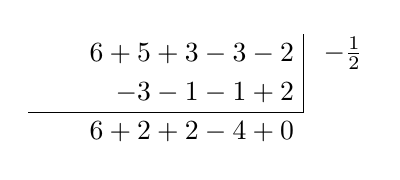
\begin{tikzpicture}
    \node at (0,0)[left]{$6+5+3-3-2$};
    \node at (0,-.5)[left]{$-3-1-1+2$};
    \node at (0,-1)[left]{$6+2+2-4+\boxed{0}$};
    \draw (-3.5,-.75)--(0,-.75)--(0,.25);
    \node at (.5,0){$-\frac{1}{2}$};
\end{tikzpicture}
\end{center}
所以$-\frac{1}{2}$是$f(x)$的根,由因式定理可得
\[f(x)=\left(x+\frac{1}{2}\right)(\poly{6,2,2,-4})\]

令$f_1(x)=\poly{6,2,2,-4}$,则$f(x)=\left(x+\frac{1}{2}\right)\cdot f_1(x)$

对$f_1(x)$求有理根,试除后知$f\left(\pm\frac{1}{3}\right)\ne 0$,因而$\pm\frac{1}{3}$不是$f_1(x)$的根,当然也不是$f(x)$的根,再用$\frac{2}{3}$试除:
\begin{center}
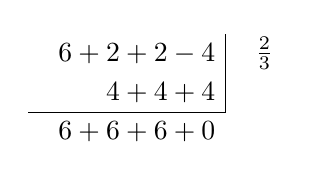
\begin{tikzpicture}
    \node at (0,0)[left]{$6+2+2-4$};
    \node at (0,-.5)[left]{$4+4+4$};
    \node at (0,-1)[left]{$6+6+6+\boxed{0}$};
    \draw (-2.5,-.75)--(0,-.75)--(0,.25);
    \node at (.5,0){$\frac{2}{3}$};
\end{tikzpicture}
\end{center}
所以$\frac{2}{3}$是$f_1(x)$的根,也就是$f(x)$的又一个根,因此
\[\begin{split}
    f(x)&=\left(x+\frac{1}{2}\right)\left(x-\frac{2}{3}\right)(\poly{6,6,6})\\
    &=6\left(x+\frac{1}{2}\right)\left(x-\frac{2}{3}\right)(\poly{1,1,1})
\end{split}\]

这里由于$x^2+x+1$的判别式$\Delta<0$, 因而它没有实数根,更不会有有理根,所以$f(2)$的有理根为$-\frac{1}{2}$, $\frac{2}{3}$。
\end{solution}

\begin{ex}
\begin{enumerate}
    \item 求$f(x)=6x^5+19x^4+22x^3+23x^2+16x+4$的有理根。
    \item 证明:多项式$f(x)=a_nx^n+a_{n-1}x^{n-1}+\cdots+a_1x+a_0$有根1的必要充分条件是
    \[ a_n+a_{n-1}+\cdots +a_1+a_0=0\]
\end{enumerate}
\end{ex}

\subsection{多项式的正根与负根}

对于实系数多项式
\[f(x)=a_nx^n+a_{n-1}x^{n-1}+\cdots+a_1x+a_0,\qquad (a_n\ne 0)\]
的根,我们有以下判定有、无正根或负根的定理:

\begin{blk}{定理3}
    如果实系数多项式
    \[f(x)=a_nx^n+a_{n-1}x^{n-1}+\cdots+a_1x+a_0,\qquad (a_n\ne 0)\]
    的各项系数$a_i,\; (i=n,n-1,\ldots,1, 0)$都是非负数,那么这个多项式$f(x)$就没有正数根。
\end{blk}

\begin{proof}
(用反证法)若$\alpha>0$且$f(\alpha)=0$, 则
\[a_n\alpha^n+a_{n-1}\alpha^{n-1}+\cdots+a_1\alpha+a_0=0\]

等号左边全是非负数,但由已知其中至少有首项系数不为零,所以它们的和不可能为零,而等号右边为零。这是不可能的。所以$f(\alpha)=0$不成立,即$f(x)$没有正根。

由于$-f(x)$与$f(x)$有完全相同的根,所以把“$a_n,a_{n-1},\ldots,a_1,a_0$全是非负数”改为“$a_n,a_{n-1},\ldots,a_1,a_0$全是非正数”,则结论不变。
\end{proof}

这样一来,如果要求一个各项系数符号统一的多项式的根,就可以不考虑正根了。如练习中的1肯定不会有正根。

\begin{blk}{定理4}
     如果实系数多项式
 \[f(x)=a_nx^n+a_{n-1}x^{n-1}+\cdots+a_1x+a_0,\qquad (a_n\ne 0)\]
偶次项系数都为非负(或非正)数,而奇次项系数又都为非正(或非负)数。那么这个多项式$f(x)$就没有负根。
\end{blk}

同学们可以自己用反证法证明这个定理。

有了这两个定理,配合定理1, 2就可以进一步缩小求有理根时试除的范围。

\begin{example}
    求$f(x)=5x^6-7x^5-8x^4-x^3+7x^2+8x+4$的有理根。
\end{example}

\begin{solution}
$f(x)$可能有的有理数根是$\pm 1,\pm 2,\pm 4,\pm \frac{1}{5},
\pm \frac{2}{5}, \pm \frac{4}{5}$.

用$x-1$试除得 $f(1)=0$, 因而有
\[f (x) = (x-1) (5x^5-2x^4-10x^3-11x^2-4x+4)=(x-1) f_1(x)\]
$f_1(x)$可能有的有理数根还是那几个,但再用$x-1$ 试除
$f_1(x)$, 不能整除,用$x-2$试除$f_1(x)$, 得$f_1(2)=0$, 因而有
\[f_1 (x) = (x-2) (5x^4+8x^3+6x^2+x-2)=(x-2)f_2(x)\]
$f_1(x)$所没有的根,$f_2(x)$当然也不会有。因此,$f_2(x)$可能有的有理数根是$-1,\pm 2,\pm \frac{1}{5},\pm \frac{2}{5}$. 但再用$x-2$试除$f_2(x)$不能整除,说明$f_2(x)$已没有正整数根;用$5x-1$试除$f_2(x)$不能整除,再用$5x-2$试除$f_2(x)$, 得$f_2\left(\frac{2}{5}\right)=0$, 
因而又有
\[f_2 (x) = (5x-2) (x^3+2x^2+2x+1)=(5x-2)f_3(x)\]
$f_3(x)$已没有正根,可能有的负根只是$x=-1$; 用$x+1$试除$f_3(x)$得$f_1(-1)=0$, 因而有
\[f_5 (x) = (x+1) (x^2+x+1)=(x+1)f_4(x)\]
$f_4(x)$已没有实数根,因而,说明$f(x)$不再有有理数根。所
以$f(x)$的有理数的是$1, 2,\frac{2}{5},-1$.
\end{solution}

\begin{ex}
\begin{enumerate}
    \item 求$f(x)=x^3-4x^2+x+6$的有理根。
    \item 解方程$2x^4+x^3+12=7x^2+16x$(仅求有理根)。
\end{enumerate}
\end{ex}

\section*{习题4.2}
\addcontentsline{toc}{subsection}{习题4.2}
\begin{enumerate}
    \item 求下列多项式的有理根:
    \begin{multicols}{2}
  \begin{enumerate}
\item $x^3-7x+6$
\item $x^4-2x^2+3x-2$
\item $x^3-9x^2+26x-24$
\item $10x^3-9x^2-3x+2$
\item $2x^5-5x^2-2x+2$
\item $5x^4+24x^3-15x^2-118x+24$
\item $x^4-4a^3x+3a^4\quad (a\in\mathbb{Q})$
\item $x^3-ax^2-b^2x+ab^2\quad (a,b\in\mathbb{Q})$
\end{enumerate}      
    \end{multicols}
\item 分解因式:
\begin{enumerate}
    \item $6x^4+5x^3y+3x^2y^2-3xy^3-2y^4$
    \item $x^4-(a^2+b^2)x^2 +a^2b^2$
    \item $x^4-4x+3$
\end{enumerate}

\item 解下列方程:
\begin{enumerate}
    \item $4x^3-3x-1=0$
\item $8x^4-6x^3-7x^2+6x-1=0$
\end{enumerate}

\item 试证明:$-1$为多项式$f(x)$的根的必要充分条件是$f(x)$的奇次项系数之和等于$f(x)$的偶次项系数之和。

\item 证明:$f(x)=2x^3+2x-1$ 没有有理根。
\item 求$g(x)=2x^5+3x^4-15x^3-26x^2-27x-9$的有理根,并分解因式。
\end{enumerate}
    
\section{两个多项式的公根与多项式的重根}
公根和重根的问题,也是多项式理论中的基本问题,特别是多项式的重根问题,在下一节实根的讨论与计算中将起重要作用。

\subsection{两多项式的公根} 
设多项式$f(x)$与$g(x)$都有一个根$\alpha$, 即$f(\alpha )=0$, $g(\alpha )=0$, 则$\alpha$ 就叫做多项式$f(x)$与$g(x)$的公根。

由因式定理可以知道,多项式$f(x)$有一个根$\alpha$ 的充要条件是$f(x)$含有一次因式$x-\alpha$.

因此,对于两个多项式$f(x)$, $g(x)$的公根$\alpha$, 就有以下定理:

\begin{blk}{定理1}
    两多项式$f(x)$, $g(x)$有一个公根的必要充分条件是这两个多项式必有一个一次公因式。
\end{blk}

\begin{proof}
    必要性。设$f(x)$, $g(x)$有一个公根$\alpha$, 则由因式定理得
\[f (x) = (x-\alpha ) \cdot f_1 (x),\qquad g(x)=(x-\alpha )\cdot g (x)\]
显然,$f(x)$, $g(x)$有一次公因式 $x-\alpha$。

充分性。设$f(x)$, $g(x)$有一公因式$x-\alpha$, 则有
\[f (x) = (x-\alpha ) \cdot f_1 (x),\qquad g (x) = (x-\alpha ) \cdot g_1 (x)\]
显然就有$f(\alpha )=0$, $g(\alpha )=0$. 所以,
$\alpha$ 就是$f(x)$, $g(x)$的一个公根。

又由于两个多项式的公因式都是它们的最高公因式的因
式,因此,两多项式的公根必定都是它们的最高公因式的根。反之,两多项式的最高公因式的根也必定是这两个多项式的公根。

这样一来,要求两个多项式的公根,只要先求出它们的最高公因式,再求这一公因式的根就可以了。
\end{proof}

\begin{example}
    求$f(x)=2x^3+x^2-5x-3$与$g(x)=2x^3-5x^2+x+3$的公根。
\end{example}

\begin{solution}
    先用辗转相除法求得$\big(f (x) ,g (x) \big) =x^2-x-1$
    这一多项式的根为$a=1\pm\frac{\sqrt{5}}{2}$. 所以$f(x)$与$g(x)$的公根为
\[x_1=1+\frac{\sqrt{5}}{2},\qquad x_2=1-\frac{\sqrt{5}}{2}\]
    
    如果能通过确定每个多项式有理根的范围首先将多项式进行因式分解,那么也一样可以求得两多项式的公根,这样也就省去辗转相除求最高公因式的繁杂计算了。

    还可以先求出一个多项式的根,再去逐个代入另一多项式进行检验,凡能使第二个多项式的值为0的,就是公根;否则就不是。
\end{solution}

\begin{example}
    试求$f(x)=ax^2+bx+c$与$g(x)=x^2-1$有一个公根的必要条件。
\end{example}

\begin{solution}
    因为$g(x)=x^2-1=(x+1)(x-1)$, 所以
    $g(x)$有两个根$1,-1$, 因此,$f(x)$与$g(x)$有一个公根只可能是1或$-1$。

若公根为1, 则$a+b+c=0$;若公根为$-1$, 则$a-b+c=0$。所以$f(x)$与$g(x)$有一个公根的必要条件是
\[a+b+c=0\quad \text{或}\quad a-b+c=0\]
\end{solution}

\begin{ex}
    \begin{enumerate}
        \item 试求$f(x)=4x^4+26x^4+51x^3-7x-24$与
$g(x)=3x^4+20x^3+32x^2-8x-32$的公根。
\item 试求$f(x)=4x^5-5x^4+1$与$g(x)=x^4-4x+3$的公根。
\item 如果$f(x)=x^2+kx+1$与$g(x)=x^2+x+k$且$k\ne 1$,
并已知它们只有一个公根。试求$k$的值及这一公根的值。
    \end{enumerate}
\end{ex}

\subsection{多项式的重根}

对于多项式$f(x)$, 如果有$f(x)=(x-\alpha )^m\cdot q(x)$,且$q(\alpha )\ne 0,\; (m>1\in\mathbb{Z})$。
那么,我们就说$\alpha$ 是$f(x)$的$m$重根。

重根的判定和排除,是计算多项式的实数根时很注重的问题。在此,我们给出以下定理。

\begin{blk}{定理2}
    如果$\alpha$ 是多项式$f(x)$的$m$重根($m>1$),那么$\alpha$ 必定是$f'(x)$的$m-1$重根。
\end{blk}

\begin{proof}
    由定理条件知$f(x)=(x-\alpha )^m\cdot q(x)$且$q(\alpha )\ne 0$, 又由多项式乘积的求导数公式,得
\[\begin{split}
     f' (x) &=m (x-\alpha )^{m-1}\cdot q (x) + (x-\alpha )^m\cdot q'(x)\\
&=(x-\alpha ) ^{m-1}\cdot  [mq (x) + (x-\alpha ) q' (x) ]
\end{split}\]
其中由于$q(\alpha )\ne 0$, $m>1$, 因而$m\cdot q(\alpha )\ne 0$,所以$\alpha$ 就是$f'(x)$的$m-1$重根。
\end{proof}

\begin{blk}{定理3}
    $\alpha$ 是多项式$f(x)$的二重根的必要充分条件是$\alpha$ 为$f(x)$与$f'(x)$的公根,且$f''(\alpha )\ne 0$。
\end{blk}

\begin{proof}
    必要性:由泰勒公式,得
\begin{equation}
    f(x)=f(\alpha)+\frac{f'(\alpha)}{1!}(x-\alpha)+\frac{f''(\alpha)}{2!}(x-\alpha)^2+\cdots+\frac{f^{(n)}(\alpha)}{n!}(x-\alpha)^n
\end{equation}
由于$\alpha$ 是$f(x)$的二重根,根据因式定理,得
\[(x-\alpha )^2|f (x) \]
因而有:
$f (\alpha ) +\frac{f' (\alpha )}{1!} (x-\alpha )=0$。

所以,$f(\alpha )=f'(\alpha )=0$, 且$f''(\alpha )\ne 0$, $\alpha$ 是$f(x)$, $f'(x)$的公根,对任意$x$都成立。

充分性:由$f(x)$,$f'(x)$有公根$\alpha$, 且$f''(\alpha )\ne 0$,则$f(\alpha)= 0$,$f'(\alpha)=0$。再从泰勒公式(4.12)不难得出
\[(x-\alpha )^2|f (x) \]
所以,$\alpha$是$f(x)$的二重根。
\end{proof}

定理3完全可以类似地推广到m重根的情形,得到下述定理:

\begin{blk}{定理4}
    $\alpha$ 是$f(x)$的$m$重根的必要充分条件是$\alpha$ 是$f(x),f'(x),\ldots,f^{(m-1)}(x)$的公根,且$f^{(m)}(\alpha )\ne 0$。
\end{blk}

如果再结合定理1、2的内容,我们就可以得出:要判定
$f(x)$有没有重根,只要看$f'(x)$, $f(x)$的最高公因式就可以了,若最高公因式含有因式$(x-\alpha )^{m-1}$, 则可以断定$f(x)$有$m$重根$\alpha$, 同时还可以断定$f'(x)$有$m-1$重根$\alpha$, $f''(x)$有$m-2$重根$\alpha,\ldots$


\begin{example}
    试求$f(x)=\poly{1,-3,2,2,-3,1}$的重根。
\end{example}

\begin{solution}
    先求出导数$f' (x) =5x^4-12x^3+6x^2+4x-3$,
再用辗转相除法求出
\[\big(f (x) ,f' (x) \big) =x^3-3x^2+3x-1= (x-1)^3\]
所以,
\[(x-1)^3|f(x),\qquad (x-1)|f'(x)\]
即$x=1$是$f(x)$与$f'(x)$的公根。因此,$f(x)$有重根1(而且是$f(x)$的4重根,$f'(x)$的3重根)。
\end{solution}

\begin{example}
  求证方程$x^4+2x^3-15x^2+4x+20=0$
有二重根,并求出这个方程的根。  
\end{example}

\begin{solution}
 设$f(x)=x^4+2x^3-15x^2+4x+20,\quad 
f' (x) =4x^3+6x^2-30x+4$,
由辗转相除法可求出$\big(f(x),f'(x)\big)=x-2$, 这是一次式。
所以,$f(x)$有二重根2, 也就是原方程有二重根2, 再用因式定理,得:
\[f (x) = (x-2)^2  (x^2+6x+5)= (x-2)^2 (x+1)(x+5)\]
因此,原方程可变形为
\[(x-2)^2 (x+1)(x+5)=0\]
所以原方程的各根为:$2, 2,-1,-5$.   
\end{solution}

\begin{ex}
    \begin{enumerate}
        \item 判定下列多项式是否有重根?若有,试求出重根来:
\begin{enumerate}
    \item $f(x)=\poly{1,-4,0,8,4}$
    \item $g(x)=\poly{4,8,-8,3}$
\end{enumerate}
        \item 举例说明定理2的逆命题是不正确的。
    \end{enumerate}
\end{ex}

\section*{习题4.3}
\addcontentsline{toc}{subsection}{习题4.3}
\begin{enumerate}
\item 求下列各组多项式的公根:
\begin{enumerate}
    \item $f (x) =x^3+5x^2+3x-9,\qquad 
g (x) =x^3+7x^2+15x+9$
\item $f (x) =x^3+3x^2-2x-6,\qquad 
g (x) =x^3-3x^2-2x+6$
\item  $f (x) =x^4-5x^2+4,\qquad g (x) =x^2+x-2$
\end{enumerate}


\item 已知$f(x)=2x^2-(3m+2)x+12$与$g(x)=4x^2-(9m-2)x+36$有一个公根,试求$m$的值。
\item 求下列多项式的重根:
\begin{enumerate}
    \item $f (x) =9x^3+12x^2-11x+2$
    \item $f(x)=\poly{1,0,4,-4,-3}$
    \item $f (x) =x^4-2x^3-x^2-4x+12$
    \item $g (x) =x^5-5x^4+7x^3-2x^2+4x-8$
\end{enumerate}

\item 若多项式$f(x)=x^3-12x+a$有重根,试求$a$.
\item 试求多项式$g(x)=x^4-px^2+q$有重根的必要条件
\item 已知多项式$f(x)=\poly{1,-1,-3,4,-4}$有两个互为相
反数的根,试求出这两个根。
\item 试一试,举例验证:如果多项式$f(x)$有重根,那么多
项式$g(x)=\frac{f(x)}{\bigl(f (x) ,f' (x)\bigr)}$就没有重根,但$g(x)$与$f(x)$
有相同的根。
\end{enumerate}


\section{实系数多项式的实数根}
对于实系数多项式
\[f(x)=a_nx^n+a_{n-1}x^{n-1}+\cdots+a_1x+a_0,\qquad (a_n\ne 0)\]
的根的讨论,要困难和复杂得多,因为多项式的根除了有理根之外,更多的是存在无理数根,而且五次以上的多项式,求根公式根本没有。因此,如何求出这些多项式的实根(如果存在的话)?特别是如何求出这些多项式的无理根的近似值?就成为我们急需讨论的内容了。

\subsection{计算实根近似值的基本思想}
求实系数多项式的实
根的近似值,主要采用逼近法,其理论根据就是今后要详细学习的中间值定理,我们现在叙述和解释如下:

\begin{blk}{定理1(中间值定理)}
    $f(x)$是一个实系数的多项式,$a<b$。若$f(a)$
    与$f(b)$符号相反,则一定存在一实数$c$,$a<c<b$使$f(c)=0$.
\end{blk}

我们从图象上来解释中间值定理。如图4.1, 由于$f(a)$
与$f(b)$符号相反,所以点$\big(a,f(a)\big)$及点$\big(b,f(b)\big)$分别在$x$轴的两侧,而曲线$y=f(x)$是连续的。因此它从$x$轴的一侧运动到$x$轴的另一侧,至少要“穿过”$x$轴一次。若在$(c,0)$点穿过,就有$f(c)=0$.

\begin{figure}[htp]
    \centering
\begin{tikzpicture}[>=latex]
    
\end{tikzpicture}
    \caption{}
\end{figure}

这样的解释尽管是直观形象的,但还不能算是严格证明。因为:什么叫连续?为什么多项式函数在$(-\infty,+\infty)$是连续的?这些问题还没有确切的交待过。而且对于一般连续函数的这一中间值定理,我们也不满足于仅仅是几何解释。不过我们目前只是直观承认这一条定理的内容并初步应用它。以后在微积分学习中再详细证明。

\begin{example}
    判断多项式$f(x)=\poly{1,0,-3,1}$的实根介于哪些连续整数之间?
\end{example}

\begin{solution}
显然,当$x\le -3$时,$f(x)<0$, 且有:
\[f (-2) =-1,\qquad f (-1) =+8,\qquad f (0) =+1,\qquad f (1)=-1,\qquad f(2)=+3\]

$x>3$时,$f(x)>0$。

所以$f(x)$在$(-2,-1)$, $(0, 1)$及$(1, 2)$各有一实根。
\end{solution}
    
例4.14说明了中间定理的作用,但并没有告诉我们多项式实根如何定位的基本方法。因为尽管在这一题中,$f(-2)$, $f(-1)$, $f(0)$, $f(1)$, $f(2)$求出后,实根的位置是显然的,但是怎样想到用$-2,-1, 0, 1, 2$的函数值作为试探的目标呢?万一$f(x)$的根是一个很大的数,例如$10^6$左右的数时,岂不要试上$10^6$个函数值?万一$f(x)$只有一个实数根,再找另两个根时不仅徒劳,而且不知到什么时候才能明确另两个不是实根。何况还可能有一些多项式根本没有实根。

这样看来,要寻求求多项式实根近似值的更完善的途径,必须解决以下三个问题:
\begin{enumerate}
\item 确定根的界限——求出一个区间,使多项式的实根在
这一范围内;    
\item 根的分离定位——判定多项式的实根的个数,并使每
个实根只包含在一个小区间内;    
\item 根的计算——求出每一实根的近似值。
\end{enumerate}

本节将系统解决这些问题,在着手解决这些问题之前,我们首先要明确逼近法的基本思想,即如何计算出$f(x)$在$(a,b)$中的一个实根的近似值?使它能达到指定的精确度?

\begin{example}
    求$f(2)=x^3-3x+1$在$(1, 2)$中的实根的近似值。(要求误差不超过0.001)
\end{example}

\begin{solution}
    由中间值定理可知,在$(1, 2)$中$f(x)$有一个实根,设为$\alpha$,为了求出要求精度范围内的近似值,可以把区间$(1, 2)$十等分,将分点$1.1,\; 1.2,\ldots,\; 1.8,\; 1.9$分别代入$f(x)$, 由于$f(1. 5)=-0.125$, $f(1. 6)=+0.296$, 所以这个根$\alpha$在$(1.5, 1. 6)$中,即$\alpha$精确到0.1的不足近似值为1.5。
    
    再把区间$(1.5, 1. 6)$十等分,将分点$1.51,\; 1.52,\ldots,\; 1.58, 1.59$分别代入$f(x)$, 因为$f(1.53)=-0.008423$, $f(1.54)=+0.03226$,所以这个根$\alpha$在$(1.53, 1. 54)$中,即$\alpha$精确到0.01的不足近似值为1.53。

    继续将$(1.53, 1.54)$十等分,计算各分点的多项式的值,因为$f(1. 532)=-0. 00010$, $f(1. 533)=+0.00369$, 所以,根$\alpha$在$(1. 532, 1. 533)$中,它的精确到0.001的不足近似值为$\alpha\approx1.532$.

    如果继续这样做下去,只要细心、不嫌繁,就可以求出
    精确到任意水平的根的近似值。
\end{solution}

    例4.15说明是逼近法的基本思想,也是求实根的基本方法,它的主要依据就是中间值定理。但方法繁,计算量大,现在已有不少更先进的算法,我们将在后边介绍一种改进了的方法。

\begin{ex}
\begin{enumerate}
    \item 利用中间值定理,判定下列多项式的实根在哪些连续整
数之间:
\begin{enumerate}
    \item $f (x) =x^4-6x^3+5x^2+12x-6$
    \item $f (x) =2x^3-5x^2+5x-3$
\end{enumerate}
\item 利用逼近法,试求$f(x)=x^3-8x+1$在$(0, 1)$中的实
根,(精确到0.001)
\end{enumerate}
\end{ex}

\subsection{实系数多项式实根的界和定位}

我们已经知道,根
据中间值定理,可以经过耐心细致的计算,首先确定多项式实根的位置在哪些连续整数之间,其次再用逼近法去求每一个实根的近似值。但是,对某一些多项式,如果我们一开
始就用一个整数进行试算,可能会发生困难,一则难在应从哪一个整数试起呢?二则难在有些多项式用整数试算找不到实根存在的区间,中间值定理无能为力。

\begin{example}
   试判定下列多式项的实根在哪两个连续整数之间?
\begin{multicols}{2}
 \begin{enumerate}
     \item $f (x) =x^4-6x^2+10$
     \item $g(x)=8x^2-8x+1$
 \end{enumerate}
\end{multicols}
\end{example}

\begin{solution}
\begin{enumerate}
    \item 由于$f(x)=(x^2-3)^2+1$, 因此,无论用那一个整数$a$去试算,恒有$f(a)>0$, 中间值定理无法判断。
    
    实际上,$f(x)$确实没有实根。
    \item 一方面当我们用一个个
    整数$a$试算$g(a)$的值时,会发现总有$g(a)>0$, 好像可以断言$g(x)$没有实根了;但另一方面,
    用求根公式可以求得$g(x)$的两个根:
    $x=\frac{2\pm\sqrt{2}}{4}$,
    显然都是实根。只不过这两个实根都在$(0, 1)$中间,其图象如图4.2所示。

    这样看来,尽管$g(0)>0$, $g(1)>0$是同号的,但在$(0, 1)$中不是没有实根,而是有两个实根。
\end{enumerate}

\begin{figure}[htp]
    \centering
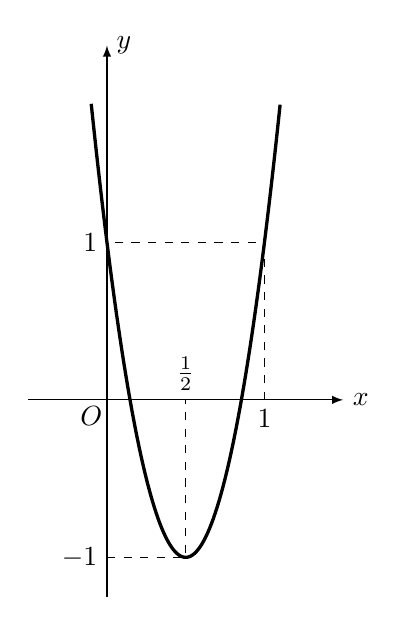
\begin{tikzpicture}[>=latex, scale=2]
\draw[->] (-.5,0)--(1.5,0)node[right]{$x$};
\draw[->] (0,-1.25)--(0,2.25)node[right]{$y$};
\node at (-.1,-.1){$O$};
\draw[domain=-.1:1.1, samples=100, very thick]plot(\x, {8*\x*\x-8*\x+1});
\draw [dashed](0,-1)node[left]{$-1$}--(.5,-1)--(.5,0)node[above]{$\frac{1}{2}$};
\draw [dashed](1,0)node[below]{$1$}--(1,1)--(0,1)node[left]{1};

\end{tikzpicture}
    \caption{}
\end{figure}
\end{solution}

这就提醒我们注意,中间值定理所述的内容中$f(a)$与$f(b)$符号相反只是$f(x)$在$(a,b)$中有实根的充分条件,但不是必要条件。
    
    依据中间值定理,运用逼近法求多项式的实根时,由于会遇到以上困难,因而我们就不得不进一步来探求新的更有效的方法。史笃姆方法就是彻底解决实根个数及定位的有效方法。
    
    史笃姆方法只是对没有重根的多项式来说的,因此可设多项式$f(x)$没有重根。

又因为当多项式的首项系数$a_n\ne 1$时,可用$a_n$去除这
个多项式的每一项,从而得到一个首项系数为1的实系数多项式,它的零点(实根)不发生变化。因此,我们就可设
$f (x) =x^n+a_{n-1}x^{n-1}+\cdots +a_1x +a_0$是一个没有重根的实系数多项式。

\begin{example}
    
\end{example}

\begin{solution}
    
\end{solution}


\begin{example}
    
\end{example}

\begin{solution}
    
\end{solution}



\begin{example}
    
\end{example}

\begin{solution}
    
\end{solution}


\begin{example}
    
\end{example}

\begin{solution}
    
\end{solution}


\begin{example}
    
\end{example}

\begin{solution}
    
\end{solution}



\begin{example}
    
\end{example}

\begin{solution}
    
\end{solution}














%P286

\begin{ex}
解下列方程组
\begin{enumerate}
    \item $\begin{cases}
        \sqrt{x}+\sqrt{y}=a\\
        x\cdot y=b
    \end{cases}\quad (a>0,\; b>0)$
    \item $\begin{cases}
        x+y=12\\ \sqrt{x+2}+\sqrt{y-1}=5
    \end{cases}$
    \item $\begin{cases}
        x^2+y^2+2(x+y)=3(xy+1)\\
        2(x^2+y^2)-xy=6(x+y)-4
    \end{cases}$
\end{enumerate}
\end{ex}

\section*{习题4.5}
\begin{enumerate}
    \item 解下列方程组:
\begin{multicols}{2}
\begin{enumerate}
    \item $\begin{cases}
        xy+36=0\\x+y=5
    \end{cases}$
    \item $\begin{cases}
        x-y=7\\x^2+y^2=85
    \end{cases}$
    \item $\begin{cases}
        x^2-y^2-3x+2y=10\\x+y=7
    \end{cases}$
    \item $\begin{cases}
        (x-2)^2+(y+3)^2=9\\ 3x-2y=6
    \end{cases}$
    \item $\begin{cases}
        4x^2-9y^2=15\\ 2x-3y=5
    \end{cases}$
    \item $\begin{cases}
        \sqrt{x+1}+\sqrt{y-1}=5\\ x+y=13
    \end{cases}$
    \item $\begin{cases}
        \frac{4}{x^2}+\frac{25}{y^2}=25\\
        \frac{2}{x}+\frac{5}{y}=1
    \end{cases}$
    \item $\begin{cases}
        \frac{y}{x}+\frac{2x}{y}=3\\
        2x+3y=4
    \end{cases}$

\end{enumerate}
\end{multicols}

\item \begin{enumerate}
    \item $m$取什么值时,方程组$\begin{cases}
        y^2=4x\\y=2x+m
    \end{cases}$
有两个相等的实数解?并求出这个解。

\item 在什么情况下,关于$x,y$的方程组
$\begin{cases}
    x+y=a\\xy=b
\end{cases}$
有实数解?没有实数解?
\end{enumerate}


\item 解方程组:
\begin{enumerate}
    \begin{multicols}{2}
    \item $\begin{cases}
        x^2+y^2=5\\y^2=4x
    \end{cases}$
    \item $\begin{cases}
        x^2+y^2=101\\xy=-10
    \end{cases}$
    \item $\begin{cases}
        x^2-y^2+(x-y)-6=0\\
        x^2+2xy+y^2-25=0
    \end{cases}$
    \item $\begin{cases}
        x^2+xy+y^2=7\\
        6x^2-5xy+y^2=0
    \end{cases}$
\end{multicols}
    \item $\begin{cases}
        x^2-5xy+6y^2=0\\
        (x-4)(y-1)+(x-3)(y-2)=0
    \end{cases}$
    \item $\begin{cases}
        2x^2+27xy+6y^2-6x-21y-14=0\\
        2x^2-9xy-3y^2-6x+6y+4=0
    \end{cases}$
\end{enumerate}


\item 解方程组:
\begin{multicols}{2}
\begin{enumerate}
    \item $\begin{cases}
        (x-2)^2+(y-1)^2=25\\
        2(x-2)^2-3(y-1)^2=5
    \end{cases}$
    \item $\begin{cases}
        (x+3)^2+y^2=9\\
        9(x-2)^2+4y^2=36
    \end{cases}$
    \item $\begin{cases}
        x^2+y^2=8\\
        (x+1)^2=(y-1)^2
    \end{cases}$
    \item $\begin{cases}
        x^2-xy-2y^2+y=0\\
        x^2-xy-2y^2-3x+6y=0\\
    \end{cases}$
    \item $\begin{cases}
        x^2+y^2=x+y+20\\
        xy+10=2(x+y)
    \end{cases}$
    \item $\begin{cases}
        (x+y+1)^2+(x+y)^2=25\\
        x^2-y^2=8
    \end{cases}$
    \item $\begin{cases}
        2x^2-4xy+3y^2=36\\
        3x^2-4xy+2y^2=36
    \end{cases}$
    \item $\begin{cases}
        4x^2+9y^2=10\\
        2xy=1
    \end{cases}$
\end{enumerate}    
\end{multicols}

\item 解下列方程组:
\begin{enumerate}
    \item $\begin{cases}
      2x^2-xy-y^2+3x+2y=3\\
      x^2-3x+2=0  
    \end{cases}$
    \item $\begin{cases}
        x^2-15xy-3y^2+2x+9y-98=0\\
        5xy+y^2-3y+21=0
    \end{cases}$
    \item $\begin{cases}
        x^2+y^2+3xy-4x-4y+3=0\\
        xy+2x+2y-5=0
    \end{cases}$
    \item $\begin{cases}
        xy=3\\yz=6\\xz=2
    \end{cases}$
    \item $\begin{cases}
        \sqrt{\frac{x}{y}}+\sqrt{\frac{y}{z}}=\frac{5}{2}\\
        x+y=10
    \end{cases}$
    \item $\begin{cases}
        5x^2-6xy+5y^2=29\\
        7x^2-8xy+7y^2=43
    \end{cases}$
\end{enumerate}


\end{enumerate}

\section*{本章内容要点}


一、本章主要内容是讨论实系数多项式的根,若$\alpha$满足$f(\alpha)=0$, 则$\alpha$叫多项式$f(x)$的根,多项式$f(x)$的根就是方程$f(x)=0$的根。

二、多项式$f(x)$的求根,就是解方程$f(x)=0$. 对于一元多项式$f(x)$: 一次、二次、三次、四次多项式都有求根公式(也称为根式解),而五次以上的一元多项式没有求根公式(不存在根式解)。

三、有理系数多项式$f(x)$若有有理根$\frac{p}{q}$, $(p,q)=1$则
必定有$p$能整除常数项$a_0$, $q$能整除首项系数$a_n$. 特别地,若$f(x)$有整数根$\alpha$, 则$\alpha|a_0$. 

因此,求有理系数多项式$f(x)$的有理根时,就可以首先找出$a_n$与$a_0$的因数,配成以$a_n$的因数为分母,以$a_0$的因数为分子的各种应有形式的有理分数就是所求有理根的范围;其次再用余式定理与综合除法逐个试算,确定所求多项式的有理根,特别地,有理系数多项式的整数根,只要在$a_0$的所有因数中试算,即可确定。

四、同时满足$f(\alpha)=0$, $g(\alpha)=0$的数$\alpha$, 叫做多项式$f(x)$与$g(x)$的公根。

两多项式$f(x)$与$g(x)$有公根的充要条件是它们有一次公因式;求两多项式的公根,一般只要求它们的最高公因式的根就可以;也可以先求其中一个多项式的根,再逐个代入另一多项式去试算,凡满足的,就是公根,否则就不是公根。

五、如果$\alpha$满足
$f(x)=(x-\alpha)^m\cdot q(x)$, 且$q(\alpha)\ne 0$。那么,$\alpha$就叫做$f(x)$的$m$重根。

$\alpha$是$f(x)$的二重根的充要条件是$\alpha$为$f(x)$, $f'(x)$的公根。

若$(f(x),f'(x))$含有$(x-\alpha)^{m-1}$的因式,则$\alpha$就是$f(x)$的$m$重根,也是$f'(x)$的$m-1$重根。

对于一个多项式$f(x)$, 如果它有重根,那么,$(f(x),f'(x))$就是非零次多项式,且不为零多项式。因而。
$\frac{f (x)}{(f (x) ,f' (x) )}=\varphi(x)$就是一个没有重根的多项式,而且$\varphi(x)$与$f(x)$有相同的根。

六、实系数多项式的实根,一般是用有理数近似值表示,求实根的近似值主要依据多项式函数的中间值定理,采用逼近的方法。一般地要顺序解决以下几个问题:
\begin{enumerate}
    \item 确定根界
    
    多项式$f(x)=x^n+a_{n-1}x^{n-1}+\cdots+a_1x+a_0$的所有根在$[-M,M]$之中,$M=1+|a_{n-1}|+\cdots+|a_1|+|a_0|$;
    
    \item 确定根的个数,根的定位
    
    计算史笃姆函数序列及变号数$W(-M)$, $W(M)$, 由克笃姆定理可确定:没有重根的多项式$f(x)$在$[-M,M]$中有
    $(W(-M)-W(M))$个实根,并可将每个根限定在一个确定的区间中。
    \item 计算每一实根的近似值
    
    运用秦九韶法,可以计算出在$(a,b)$中的实根的任意精确度的近似值。在具体计算过程中,主要使用了两种变换,方便和简化了运算。
 \end{enumerate}

    七、二元二次方程组分为两种类型,第(I)类型是基础,它的求解主要是采用代入消元法;第(II)类型,我们仅讨论了一些具有特点的特殊方程组的解法,其中主要是:
    \begin{enumerate}
        \item 可转化为第(I)类型求解的方程组,其转化的主要方法是因式分解;消去二次项,消去非二次项、再分解因式,总之是降次。
        \item 可转化为含有一元方程的方程组,其转化的主要方法是消去含有某一元的各项。实际就是消元。
        \item 可用换元法解的轮换对称方程组。
\end{enumerate}

至于一般的由两个二元二次方程组的方程组,如果不具有以上这些特点,其解法繁难,我们先不予讨论。以后可以使用几何法解决。


\section*{复习题四}
\begin{enumerate}
    \item 求下列多项式的有理根:
\begin{multicols}{2}
\begin{enumerate}
    \item $\poly{1,-1,-8,12}$
    \item $\poly{1,-11,18,-8}$
    \item $\poly{1,-7,-7,43,42}$
    \item $\poly{1,0,4,8,0,32}$
    \item $\poly{1,0,-1,2,-1}$
    \item $\poly{4,0,-9,6,-1}$
\end{enumerate}
\end{multicols}

\item 如果多项式$f(x)=ax^2+bx+c$的二根之比为$\frac{2}{3}$, 求证:$6b^2=25ac$。

\item 判别下列多项式有没有重根,若有,求出其重根。
\begin{enumerate}
    \item $\poly{1,0,-24,64,-48}$
    \item $\poly{1,-5,7,-2,4,-8}$
    \item $\poly{1,0,4,-4,-3}$
\end{enumerate}

\item 证明:$f(x)=1+\frac{x}{1!}+\frac{x^2}{2!}+\cdots+\frac{x^n}{n!}$没有重根。

\item 求$f(x)=x^4+x^3-2x-4$与$g(x)=x^4-x^3+2x-4$的公
根。

\item 求多项式$x^3+px+q$有重根的条件。

\item \begin{enumerate}
    \item 若$a$为整数,但$|a|\ne 2$, 试证:多项式
$f (x) =x^2+ax+1$没有有理根。
\item 若$a,b,c$都是奇数,试证明$f(x)=ax^2+bx+c$没有整数根。
\end{enumerate}


\item $a\ne 0$, 求证多项式$f(x)=x^n-a^n$没有重根。

\item 已知$f(x)=2x^4-8x^3+19x^2-12x+24$有两个根分别是
$g(x)=x^4-2x^3+3x^2-2x+2$的两个根的2倍,求这两个根。

\item 求多项式$p(x)=x^3+2x^2-5x-7$的正根的近似值,使
误差小于$10^{-8}$.

\item 求98的5次方根,使误差小于$10^{-6}$(允许应用四位对数
表求出前若干位数字)。

\item 求多项式$f(x)=x^3+x^2+x-10^{10}$的正根的近似值,使
误差小于1.

\item 将$x^5-243$写成以$x-3$为元的多项式,将$x^3+x^2+1$写
成以$x+1$为元的多项式。

\item 应用中间值定理,写出下列各多项式的实根在哪些连续
整数之间。
\begin{enumerate}
    \item $\poly{1,-2,-1,6,2}$
    \item $\poly{1,1,-2,1}$
    \item $\poly{1,-8,14,4,-6}$
\end{enumerate}

\item 若三次多项式$f(x)=x^3-2x^2-x+3$有三个根$\alpha,\beta,\gamma$,试求下列各式的值:
\begin{enumerate}
    \item $\alpha^2+\beta^2+\gamma^2$
    \item $\alpha^3+\beta^3+\gamma^3$
    \item $(\alpha+1)(\beta+1)(\gamma+1)$
    \item $\alpha^2(\beta+\gamma)+\beta^2(\alpha+\gamma)+\gamma^2(\alpha+\beta)$
\end{enumerate}


\item 应用多项式的第一种换元变形,使
$f (x) =x^3-6x^2+5x+7$变形为$g(y)$后,$g(y)$中$y$的系数为零。
\item 应用多项式的第一种换元变形,使
$f (x) =a_nx^n+a_{n-1}x^{n-1}+\cdots +a_1x+a_0\;  (a, \ne 0)$变形为$g(y)$后,$g(y)$中$y^{n-1}$的系数为零。

\item 解方程组:
\begin{multicols}{2}
  \begin{enumerate}
\item $\begin{cases}x^{2}-x y+y^{2}=48 \\ x-y-8=0\end{cases}$
\item $\begin{cases}x^{2}+3 x y+y^{2}=1 \\ 3 x^{2}+x y+3 y^{2}=13\end{cases}$
\item $\begin{cases}x^{2}+y^{2}+4 x-2 y+3=0 \\ x^{2}+4 x y-y^{2}+10 y-9=0\end{cases}$
\item $\begin{cases}x^{2}-x y=12 \\ x y-2 y^{2}=1\end{cases}$
\item $\begin{cases}\frac{1}{x^{2}}+\frac{1}{x y}=\frac{1}{a^{2}}\\
    \frac{1}{y^{2}}+\frac{1}{x y}=\frac{1}{b^{2}}
\end{cases}$
\item $\begin{cases}x^{4}+y^{4}=97 \\ x+y=5\end{cases}$
\item $2(x-y)+x y=3 x y-(x-y)=7$
\end{enumerate}  
\end{multicols}

\end{enumerate}